\ifdefined\USERMANUAL
  \newcommand{\doctype}{BENUTZERHANDBUCH}
\else
  \newcommand{\doctype}{REFERENZKARTEN}
\fi

\maketitlepage{TAIPO}{MIDI-Erweiterung}{TAIPO_SILVER_cutout_small_2}{\doctype}

\newpage
\tableofcontents
\newpage
\part{Übersicht}
\newpage
\section{Übersicht}\label{section:installation}
\subsection{Übersicht}
\paragraph*{}
\textbf{TAIPO} MIDI-Erweiterung für The Centre ermöglicht den Anschluss von The Centre
an externe Geräte (einschließlich Computer) über ein Standard-MIDI-TRS-Typ-B-Kabel.
\subsection{Was ist in der Box}
\paragraph*{}\textbf{TAIPO} wird mit Standardzubehör geliefert. In der Box finden Sie:
\begin{enumerate}
  \item \textbf{TAIPO} Eurorack-Modul
  \item Standard-Eurorack-Stromkabel (10-Pin auf 16-Pin)
  \item MIDI-EX-Verbindungskabel zur Verbindung mit \textbf{THE CENTRE}
\end{enumerate}

\newpage
\part{Installation}
\newpage
\section{Installation}
\subsection{Installationsschritte}
\paragraph*{}
Die Installation von TAIPO folgt den Schritten zur Installation eines beliebigen Eurorack-Moduls im Gehäuse des Besitzers.

\begin{figure}[h]
  \centering
  \includegraphics[height=0.5\linewidth]{taipo_the_centre_cable_install.jpg}
  \includegraphics[height=0.5\linewidth]{taipo_cable_install.jpg}
  \caption{Kabelinstallation an beiden Enden}
  \label{fig:midsinglenote}
\end{figure}

\subsection{Wichtige Installationshinweise}
\paragraph*{}
 Bitte beachten Sie die Reihenfolge der Farben auf beiden Seiten. Die Farbreihenfolge auf der Seite von The Centre sollte von oben nach unten \textbf{SCHWARZ, ROT, GELB, GRÜN} sein und auf der TAIPO-Seite umgekehrt: \textbf{GRÜN, GELB, ROT, SCHWARZ}
\newline$\blacksquare$ WICHTIG: Auf der Seite von The Centre an den MIDI-EX-Anschluss anschließen, wie im Bild oben dargestellt. Der zweite Anschluss dient zum Verbinden des MIDI-Ausgangs von The Centre mit TWINS.

\newpage
\part{MIDI}
\newpage
\section{MIDI-Kabeltypen}
\subsection{TAIPO-Kabeltyp}
\paragraph*{}
TAIPO verwendet ein MIDI 3,5mm TRS (Tip-Ring-Shield) Kabel Typ B. Siehe: \underline{\nameref{section:cabletypeb}}
\subsection{Über das MIDI-Signal}
\paragraph*{}
Das MIDI-Signal wird über ein MIDI-Kabel unter Verwendung des Standard-RS232-Protokolls gesendet, jedoch mit einer
nicht standardmäßigen Geschwindigkeit von 31250 Baud (Bits pro Sekunde). Die elektrische MIDI-Verbindung ist
gerichtet, was bedeutet, dass die interne Pinbelegung im Kabel von Bedeutung ist, da der Strom
in eine Richtung fließt. Während dies bei Standard-MIDI-DIN-Kabeln kein Problem darstellt,
wurde es bei 3,5-mm-Klinkenkabeln (TRS) problematisch, da die Hersteller begannen, sie
unterschiedlich zu verdrahten, da kein Standard definiert war. Basierend auf diesen Verdrahtungen haben sich einige
Standards herausgebildet.
\newline$\blacksquare$ Verschiedene TRS-Standards sind nicht austauschbar und nicht kompatibel.
Um Geräte mit unterschiedlichen TRS-Standards zu verbinden, muss ein passendes Kabel verwendet werden.
\subsection{DIN-Anschluss}
Standard-MIDI-Kabel mit 5-poligem DIN-Anschluss
\subsection{TRS-Anschlusstypen}
\subsubsection{Typ-A-Anschluss}
TRS Typ A definiert die \textbf{SPITZE} (TIP) des 3,5-mm-Klinkensteckers als \textit{\textbf{Quelle}} (source) und den \textbf{RING} als \textit{\textbf{Senke}} (sink).
\newline
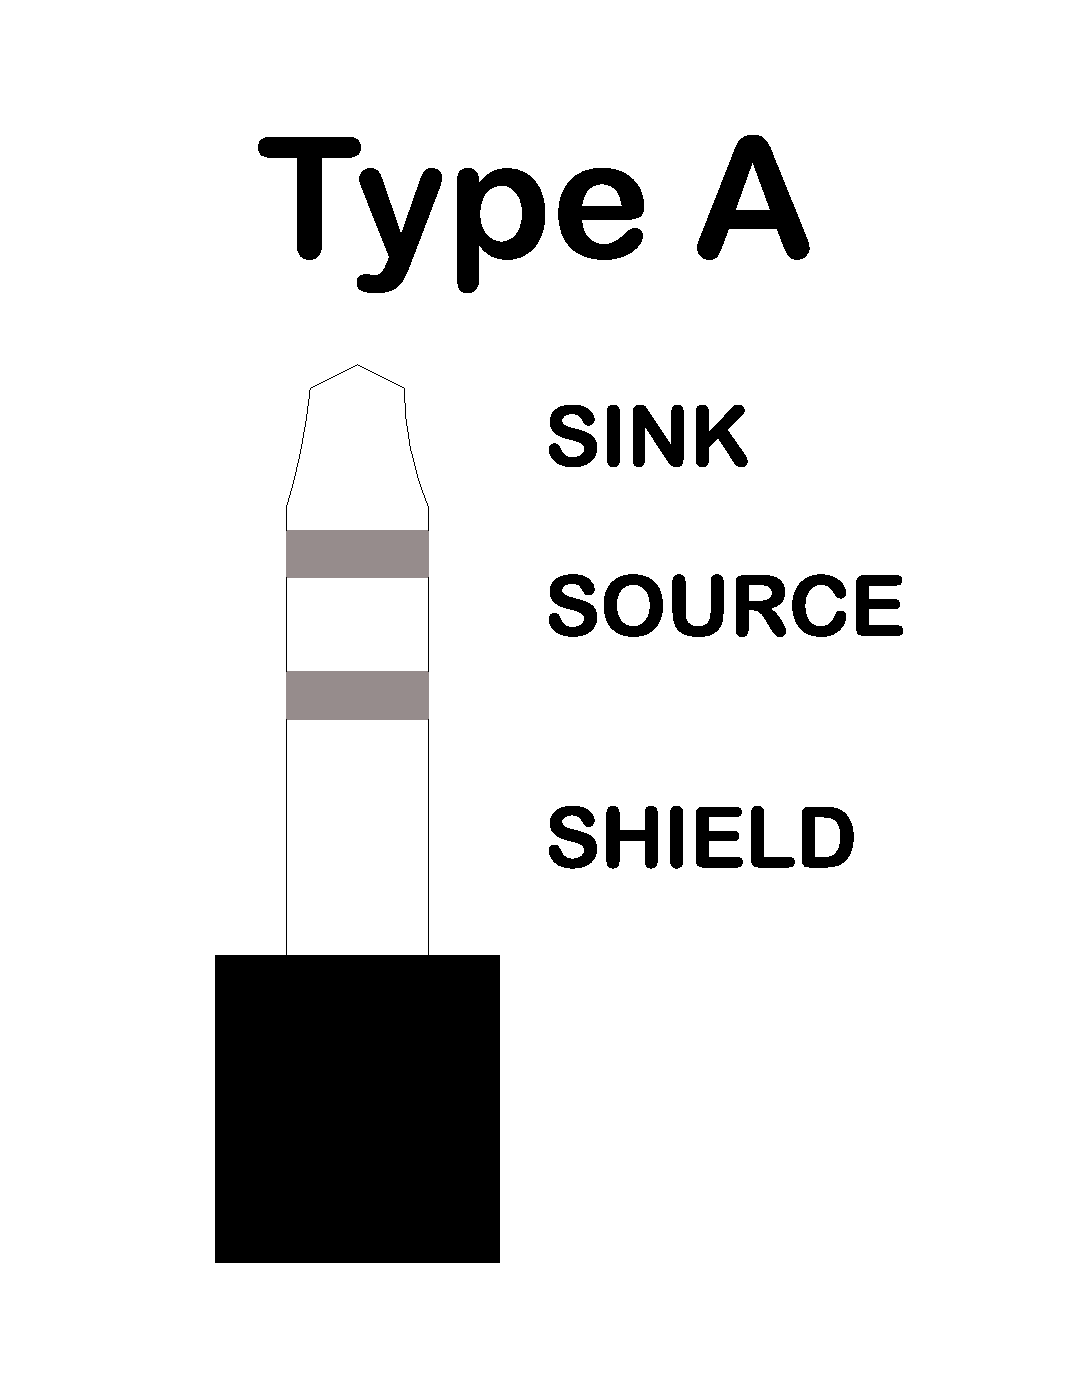
\includegraphics[height=0.3\linewidth]{midi_trs_type_a.eps}
\newline$\bigstar$ Marken, die Typ A verwenden: Korg, Akai
\subsubsection{Typ-B-Anschluss}\label{section:cabletypeb}
TRS Typ B definiert die \textbf{SPITZE} (TIP) des 3,5-mm-Klinkensteckers als \textit{\textbf{Senke}} (sink) und den \textbf{RING} als \textit{\textbf{Quelle}} (source).
\newline$\blacksquare$ Typ B ist in der Eurorack-Modular-Szene weiter verbreitet.
\newline
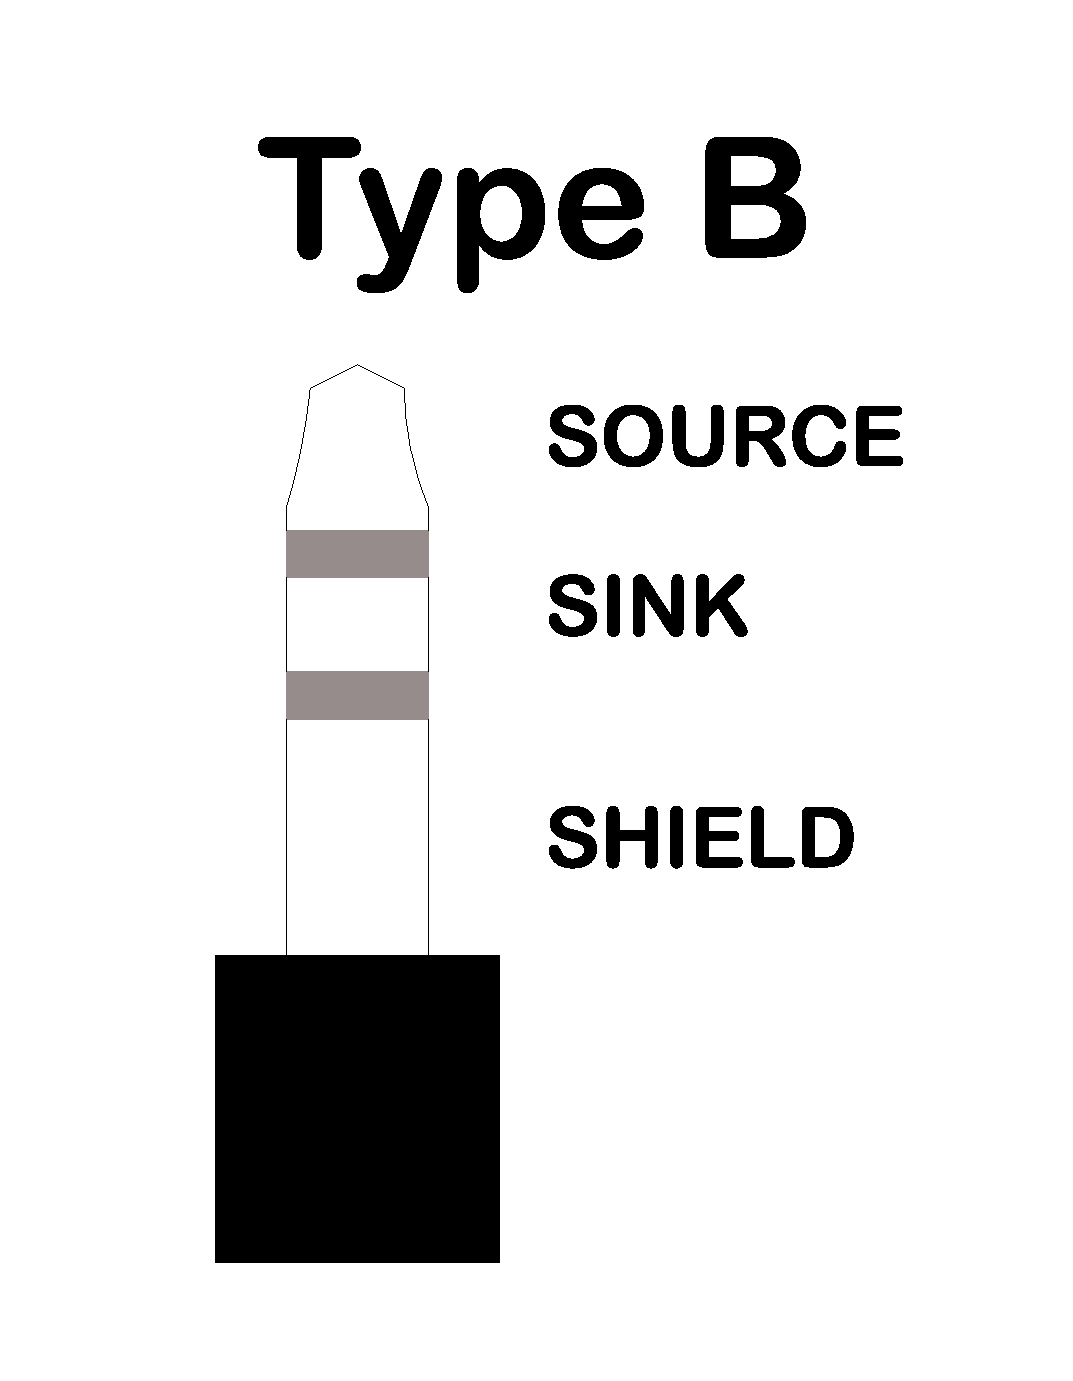
\includegraphics[height=0.3\linewidth]{midi_trs_type_b.eps}
\newline$\bigstar$ Marken, die Typ B verwenden: Arturia, Novation, 1010
